



%----------------------------------------------------------------------------------------

\newpage


\section[Existing Models][Modèles existants]{Existing Models}{Modèles existants}

\label{sec:macrocoevolexplo}

%----------------------------------------------------------------------------------------


Nous proposons dans un premier temps d'introduire les modèles de co-évolution à l'échelle macroscopique en étudiant les résultats produits par des modèles existants, ce qui permettra également d'introduire les méthodes et indicateurs d'exploration, ainsi que d'appréhender les questionnements typiques liés à ce type de modèles. En particulier, nous procédons à une exploration systématique du modele SimpopNet~\cite{schmitt2014modelisation}, initiative unique pour modéliser la co-evolution au sein d'un système de villes.



%%%%%%%%%%%%%%%%%%%%%%%
\subsection{Context}{Contexte}


\bpar{
Which differences in produced knowledge can be observed, from the conceptual or thematic description of a model, to its mathematical formalisation, its implementation, its systematic exploration, up to its exploration in deep with the help of specific meta-heuristics ? Our postulate, that is a consequence of both our positioning (see \autoref{ch:positioning} on simulation) and experiments of which previously developed models are part, is that it is considerable, but furthermore of a \emph{qualitative} nature, in the sense that the nature of knowledge follows abrupt transitions during the advance of the investigation in this continuum. The SimpopNet model introduced by~\cite{schmitt2014modelisation}, which is to our knowledge the only co-evolution model in the perspective of the evolutive urban theory, is an example of such a preliminary approach that must be explored deeper, for example through systematic exploration.
}{
Quelle différentiel de connaissances obtenues peut s'observer, de la description conceptuelle ou thématique d'un modèle, à sa formalisation mathématique, son implémentation, son exploration systématique, jusqu'à son exploration approfondie à l'aide de meta-heuristiques spécifiques ? Notre postulat, qui découle à la fois de notre positionnement (voir \autoref{ch:positioning} sur la simulation) et d'expériences dont les modèles déroulés précédemment font partie, est que celui-ci est important, mais surtout de nature \emph{qualitative}, c'est à dire que la nature même des connaissances subit des transitions abruptes lors de l'avancée de la démarche dans ce continuum. Le modèle SimpopNet introduit par~\cite{schmitt2014modelisation}, qui est à notre connaissance l'unique modèle de co-évolution dans une perspective de la théorie évolutive des villes, est un exemple d'une telle démarche préliminaire qui nécessite d'être creusée, par exemple par l'exploration systématique.
}


\paragraph{Model Description}{Description du Modèle}

Nous reformulons brièvement le modèle, en écho à la formulation du modèle d'interaction en~\ref{sec:interactiongibrat}, un certain nombre de paramètres et de processus se recoupant. Les villes croissent suivant la spécification de l'équation~\ref{eq:interactiongibrat:model}, avec $r_0 = 0$, $w_G = \lambda^\beta \cdot N$ et $V_{ij} = \mu_j / d_{ij}^\beta$. Le potentiel d'interaction ne dépend pas de la population de la ville d'origine, et le choix d'une fonction puissance permet de combiner un paramètre de décroissance $\lambda$ à un paramètre de forme $\beta$. Le réseau croît à chaque pas de temps par rupture topologique : un couple de villes est choisi, la première selon les populations avec une hiérarchie $\gamma$ (c'est à dire avec une probabilité $\mu_i^\gamma / \sum_j \mu_j^\gamma$) et la seconde selon les potentiels d'interaction $\mu_i \mu_j / d_{ij}^\beta$ avec la même hiérarchie $\gamma$, puis un lien est crée si le réseau n'est pas assez efficace, i.e. $d_{ij}/d^{(N)}_{ij}> \theta$. Les liens crées à une date $t$ ont une vitesse $v(t)$, qui dépendra des technologies de transport courantes. La planarisation n'est effectuée que pour les liens de vitesse semblable. Pour comprendre le comportement stylisé du modèle, nous considérons une configuration simplifiée telle que $v(t > t_0) = v_0$ et $v(t_0) = 1$.




\paragraph{Perspectives}{Perspectives}

Certains choix de modélisation ne sont pas en cohérence directe avec l'application qui en est faite : par exemple, une telle précision dans la paramétrisation des dates et des vitesses suggère un modèle hybride, et devrait correspondre à une application sur une configuration spatiale réelle. Dans une configuration stylisée, ces paramètres n'ont de sens que si l'on connait le comportement des dynamiques simulées, et en particulier le rôle de la configuration spatiale, c'est à dire la séparation entre effets structurels et effets conjoncturels. D'autre part, l'utilisation du modèle d'interaction sans le terme de Gibrat endogène serait difficilement adaptable pour une application du modèle sur données réelles vu les valeurs obtenues dans les études précédentes des modèles d'interaction, mais est bien cohérent dans un modèle stylisé, afin de comprendre les processus d'interaction de manière isolée, comme nous le ferons plus loin (mais en gardant à l'esprit que cette connaissance ne reflète pas nécessairement le comportement couplé, l'interaction entre les processus pouvant faire émerger de nouveaux comportements). La formulation du potentiel en $(\lambda / d_{ij})^\beta$ implique que $\lambda$ capture à la fois le poids et la décroissance, mais permet moins de liberté que la spécification que nous avon utilisé précédemment, et ne permet pas une interpretation en terme de flux limite. L'introduction de l'effet tunnel dans le modèle, via les valeurs variables de $v(t)$ et le mécanisme de non-branchement, est exogène puisque spécifié dans les règles du modèle, contrairement au modèle d'interaction avec retroaction des flux, dans lequel les variations de $w_N$ et $d_N$ doivent capturer un effet tunnel endogène. L'introduction d'indicateurs spécifiques pour le mesurer serait une piste intéressante de développement, mais nous nous contentons de regarder par exemple la hiérarchie des centralités qui en est un bon proxy.



%%%%%%%%%%%%%%%%%%%%%%%
\subsection{Methodology}{Méthode}

\subsubsection{Spatial configuration}{Configuration spatiale}

Un aspect important de la compréhension des processus de co-évolution impliqués dans ce modèle est le rôle de la configuration spatiale initiale dans les motifs émergents observés. Nous appliquons pour cela la méthodologie développée en~\ref{sec:computation}, permettant d'étendre l'analyse de sensibilité d'un modèle à des méta-paramètres spatiaux.

\paragraph{Synthetic configuration generation}{Génération de configuration synthétique}

Une système de villes synthétique, respectant au premier ordre de manière visuelle les critères de l'état initial du modèle de base, est construit de la façon suivante (voir l'Appendice~\ref{app:sec:syntheticdata} pour la notion de données synthétiques, calibrées au premier et second ordre). Une nombre fixée de villes $N$ est réparti uniformément dans l'espace conditionnellement à une distance minimale entre chaque, et leur population est attribuée suivant une loi rang-taille dont les paramètres $P_{m}$ et $\alpha$ peuvent être ajusté (la distribution du modèle initial correspond à $\alpha\simeq 0.68$ avec $R^2=0.98$). Un squelette de réseau est créé par un algorithme de connexification, qui connecte les villes deux à deux par plus proche voisins, puis itérativement sélectionne un cluster aléatoirement et le connecte perpendiculairement au lien le plus proche hors du cluster. Le réseau est ensuite étoffé par la création de raccourcis locaux, par répétitions $n_s$ fois de la selection aléatoire d'une ville selon les populations, et sa connexion à un voisin dans un rayon $r_s$ sous conditions de degré maximal $d_s$. Le réseau final est ensuite planarisé. Cette procédure crée des réseau correspondant visuellement à l'initialisation du modèle, sachant qu'une instance du réseau ne permet pas de déterminer les distributions de paramètres topologiques sur lesquels une calibration plus fine pourrait être opérée.



\paragraph{Parameters}{Paramètres}




\subsubsection{Indicators}{Indicateurs}

Un aspect toujours subtil de l'étude des modèles de simulation est la définition d'indicateurs pertinents, surtout dans le cas de modèles synthétiques où il n'est pas possible de produire des sorties directement liées aux données par exemple. Des faits stylisés très généraux, comme vouloir produire une hiérarchie urbaine ou une hiérarchie de réseau, sont relativement limités. Dans le cas de la hiérarchie particulièrement, les lois obtenues dévient d'une loi d'échelle et il est discutable d'utiliser uniquement la pente d'un ajustement brutal. De plus, la hiérarchie est produite mécaniquement par la majorité des modèles incluant des processus d'agrégation. Il faut donc des indicateurs plus élaborés pour comprendre les dynamiques du système.


Pour se concentrer sur la capacité du modèle à produire des trajectoires à la fois diverses et complexes, et par exemple sa capacité à produire des bifurcations qui se traduiraient par inversions de range, nous proposons les indicateurs suivant pour une variable $X_i(t)$ définie sur chacune des villes et dans le temps (qui pourra être la population ou des mesures de centralité par exemple) :

\begin{itemize}
  \item Indicateurs basiques : hiérarchie, entropie, statistiques descriptives, de la distribution dans le temps
  \item Corrélation de rang initial-final, qui traduit les changements dans la hiérarchie : $\rho\left[X_i(t=0),X_i(t=t_f)\right]$
  \item Diversity des trajectoires, qui capture la diversité de forme des séries temporelles, avec $\tilde{X}_i(t)\in \left[0;1\right]$ les trajectoires mises à l'échelle individuellement,
\[
\frac{2}{N\cdot(N-1)}\sum_{i<j} \left(\frac{1}{T}\int_{t} \left(\tilde{X}_i(t) - \tilde{X}_j(t)\right)^2 \right)^{\frac{1}{2}}
\]
\item Complexité moyenne des trajectoires, la ``complexité'' d'une trajectoire étant donnée simplement par son nombre de points d'inflexion
\item Corrélations en fonction de la distance, pour comprendre la manière dont l'effet de la distance est traduit au niveau macroscopique : 
\[
\hat{\rho}_d\left[(X(\vec{x}_1,Y(\vec{x}_2))|||\vec{x}_1-\vec{x}_2||\sim d\right]
\]
\item Corrélations retardées entre les variations, pour identifier des motifs de causalité entre les variables $X$ et $Y$ : \[
\hat{\rho}_{\tau}\left[\Delta X(t),\Delta Y(t-\tau)\right]
\]
\end{itemize}



Nous introduisons de plus divers indicateurs de topologie du réseau, pour comprendre les formes finales produites par l'heuristique : diamètre, longueur moyenne de chemin, centralité de chemin moyenne et niveau de hiérarchie, performance moyenne, longueur totale.




%%%%%%%%%%%%%%%%%%%%%%%
\subsection{Results}{Résultats}


\subsubsection{Experience plan}{Plan d'expérience}

Etant donne une configuration spatiale initiale (c'est a dire une valeur des meta-parametres), nous établissons les diagrammes de phase par l'exploration d'une grille de l'espace des paramètres.


\subsubsection{Model Behavior}{Comportement du modèle}


Pour comprendre la manière le modèle capture un certain ``degré de co-évolution'', les différents indicateurs de correlations sont utiles, sachant qu'au regard des travaux des chapitres précédents il s'agit une notion particulièrement subtile qui ne pourra être capturé par un indicateur unique, puisqu'on pourra s'intéresser par exemple aux régimes de causalité, aux forces de interactions en fonction de la distance, au poids de telle ou telle composante.


\subsubsection{Convergence}{Convergence}


Pour quantifier la variabilité d'un indicateur $X$ par rapport à la stochasticité, nous utilisons une mesure de type ratio de Sharpe, donnée par $v\left[X\right] = \hat{\Eb{X}}/\hat{\sigma\left[X\right]}$ avec les estimateurs basiques pour l'espérance et la deviation standard. On s'en sert egalement pour comparer la variabilité a la stochasticité a celle par rapport aux paramètres ou meta-paramètres, par exemple en calculant $v\left[X|\vec{\alpha}_1\right]/v\left[X|\vec{\alpha}_2\right]$ pour deux valeurs différentes des paramètres.





\subsubsection{Sensitivity to space}{Sensibilité à l'espace}

La table~\ref{tab:macrocoevolexplo:spacematters} donne pour les indicateurs principaux les statistiques descriptives des valeurs de $v$ au sein d'une configuration et relativement par rapport aux meta-configurations.


%%%%%%%%%%%%%
\begin{table}[!ht]
\caption[Sensibility to space][Sensibilité à l'espace]{}{\textbf{Sensibilité à l'espace du modèle SimpopNet.} Chaque colonne correspond à une instance du diagramme de phase, pour laquelle les meta-paramètres sont donnés, ainsi que la distance relative à un diagramme de référence arbitraire.\label{tab:macrocoevolexplo:spacematters}}
\begin{tabular}{|l|l|l|l|l|l|l|l|l|l|l|l|l|l|l|l|l|}
\hline
$N_S$ & 40 & 40 & 40 & 40 & 40 & 40 & 40 & 40 & 80 & 80 & 80 & 80 & 80 & 80 & 80 & 80\\
$\alpha_S$ & 0.5 & 0.5 & 0.5 & 0.5 & 1.5 & 1.5 & 1.5 & 1.5 & 0.5 & 0.5 & 0.5 & 0.5 & 1.5 & 1.5 & 1.5 & 1.5\\
$d_S$ & 5 & 5 & 10 & 10 & 5 & 5 & 10 & 10 & 5 & 5 & 10 & 10 & 5 & 5 & 10 & 10\\
$n_S$ & 10 & 30 & 10 & 30 & 10 & 30 & 10 & 30 & 10 & 30 & 10 & 30 & 10 & 30 & 10 & 30\\
$\tilde{d}$ & 0.00 & 0.29 & 0.12 & 0.29 & 1.63 & 1.75 & 1.70 & 1.63 & 0.41 & 0.43 & 0.20 & 0.38 & 2.10 & 2.13 & 2.09 & 2.04\\\hline
\end{tabular}
\end{table}
%%%%%%%%%%%%%



\subsubsection{Patterns}{Motifs}

% interesting patterns

Capable de plus de bifurcations de population et d'inversion de hierarchie que le modèle de renforcement \comment[JR]{pas sur}, car new links (varying topology) et random links. : leçon intéressante pour la dépendance au chemin. 

La Fig.~\ref{fig:macrocoevolexplo:behavior} rend compte du comportement du modèle selon les divers indicateurs donnés ci-dessus. \comment[JR]{developper brievement (deja long)}


%%%%%%%%%%%%%%%%
\begin{figure}
	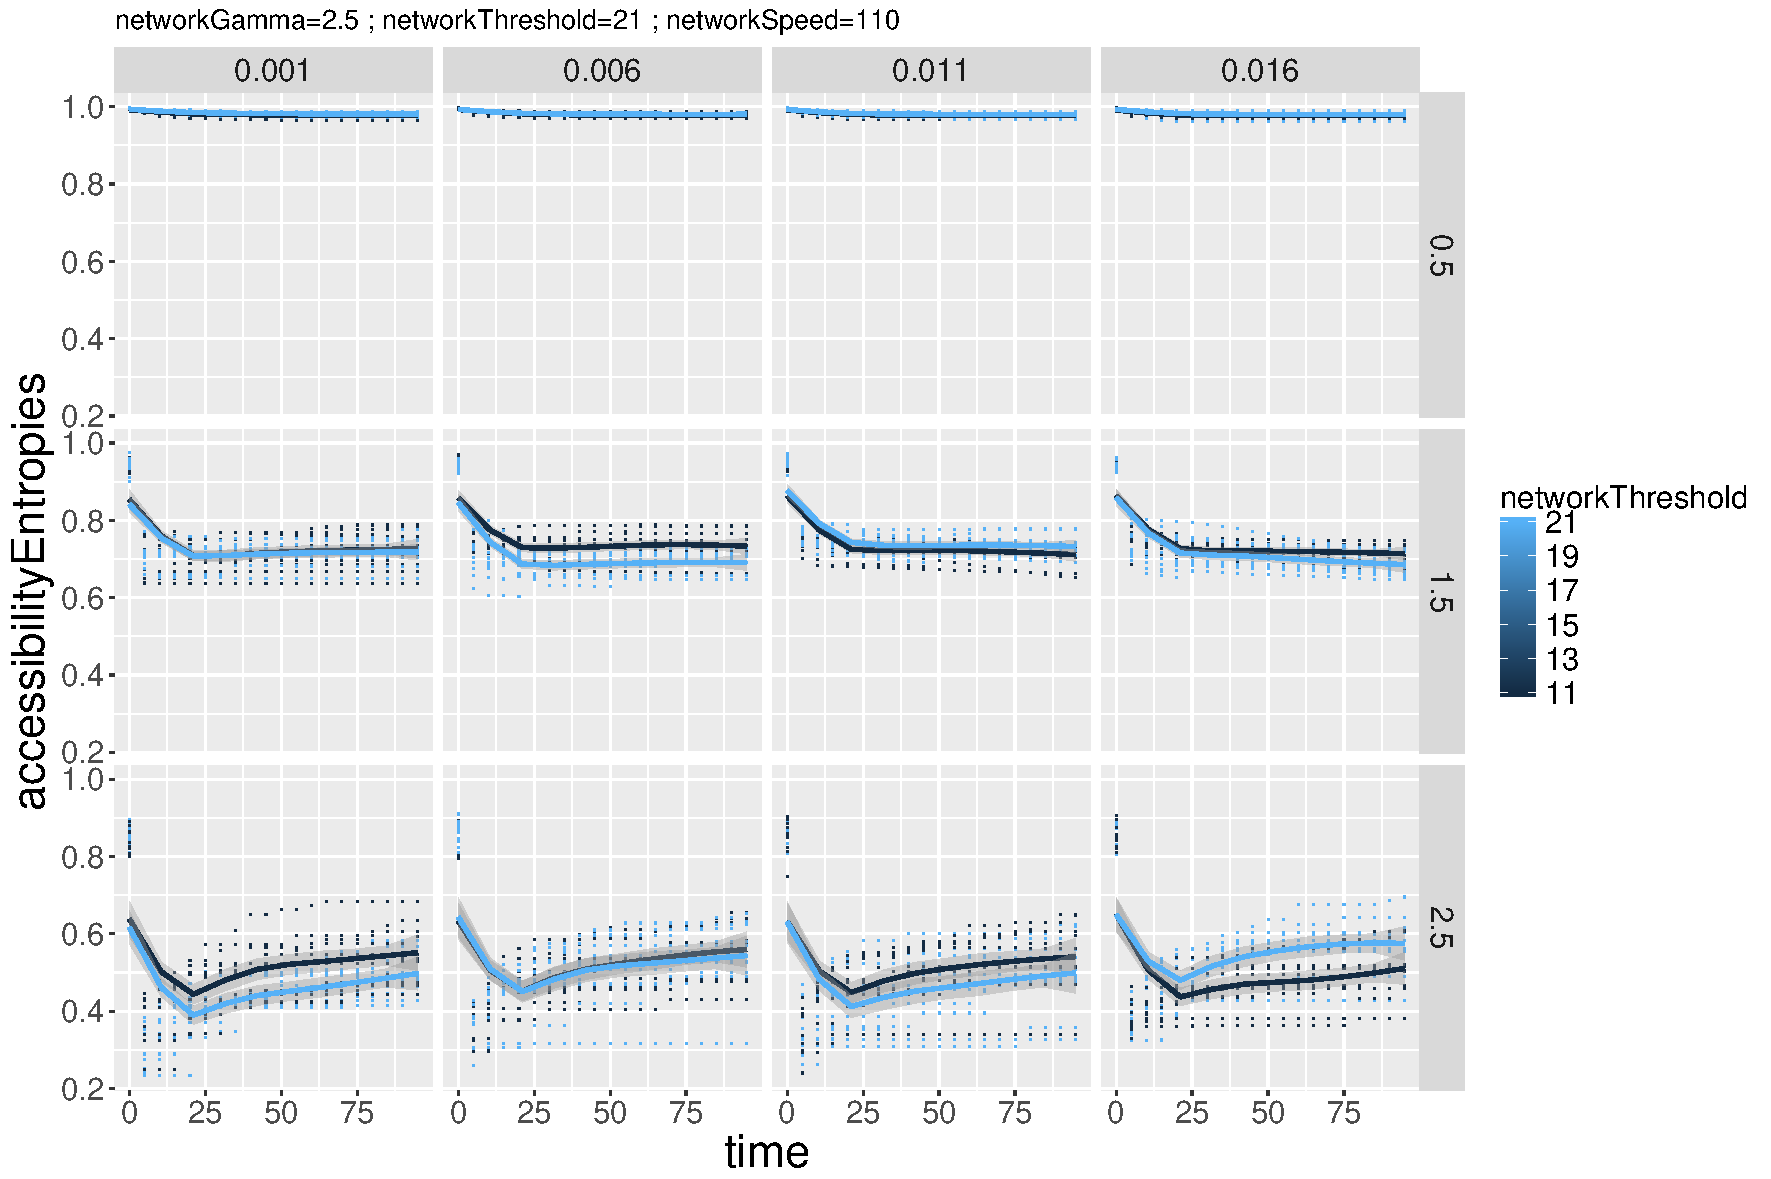
\includegraphics[width=0.48\textwidth]{Figures/MacroCoEvolExplo/accessibilityEntropies_networkGamma2_5_networkThreshold21_networkSpeed110}
	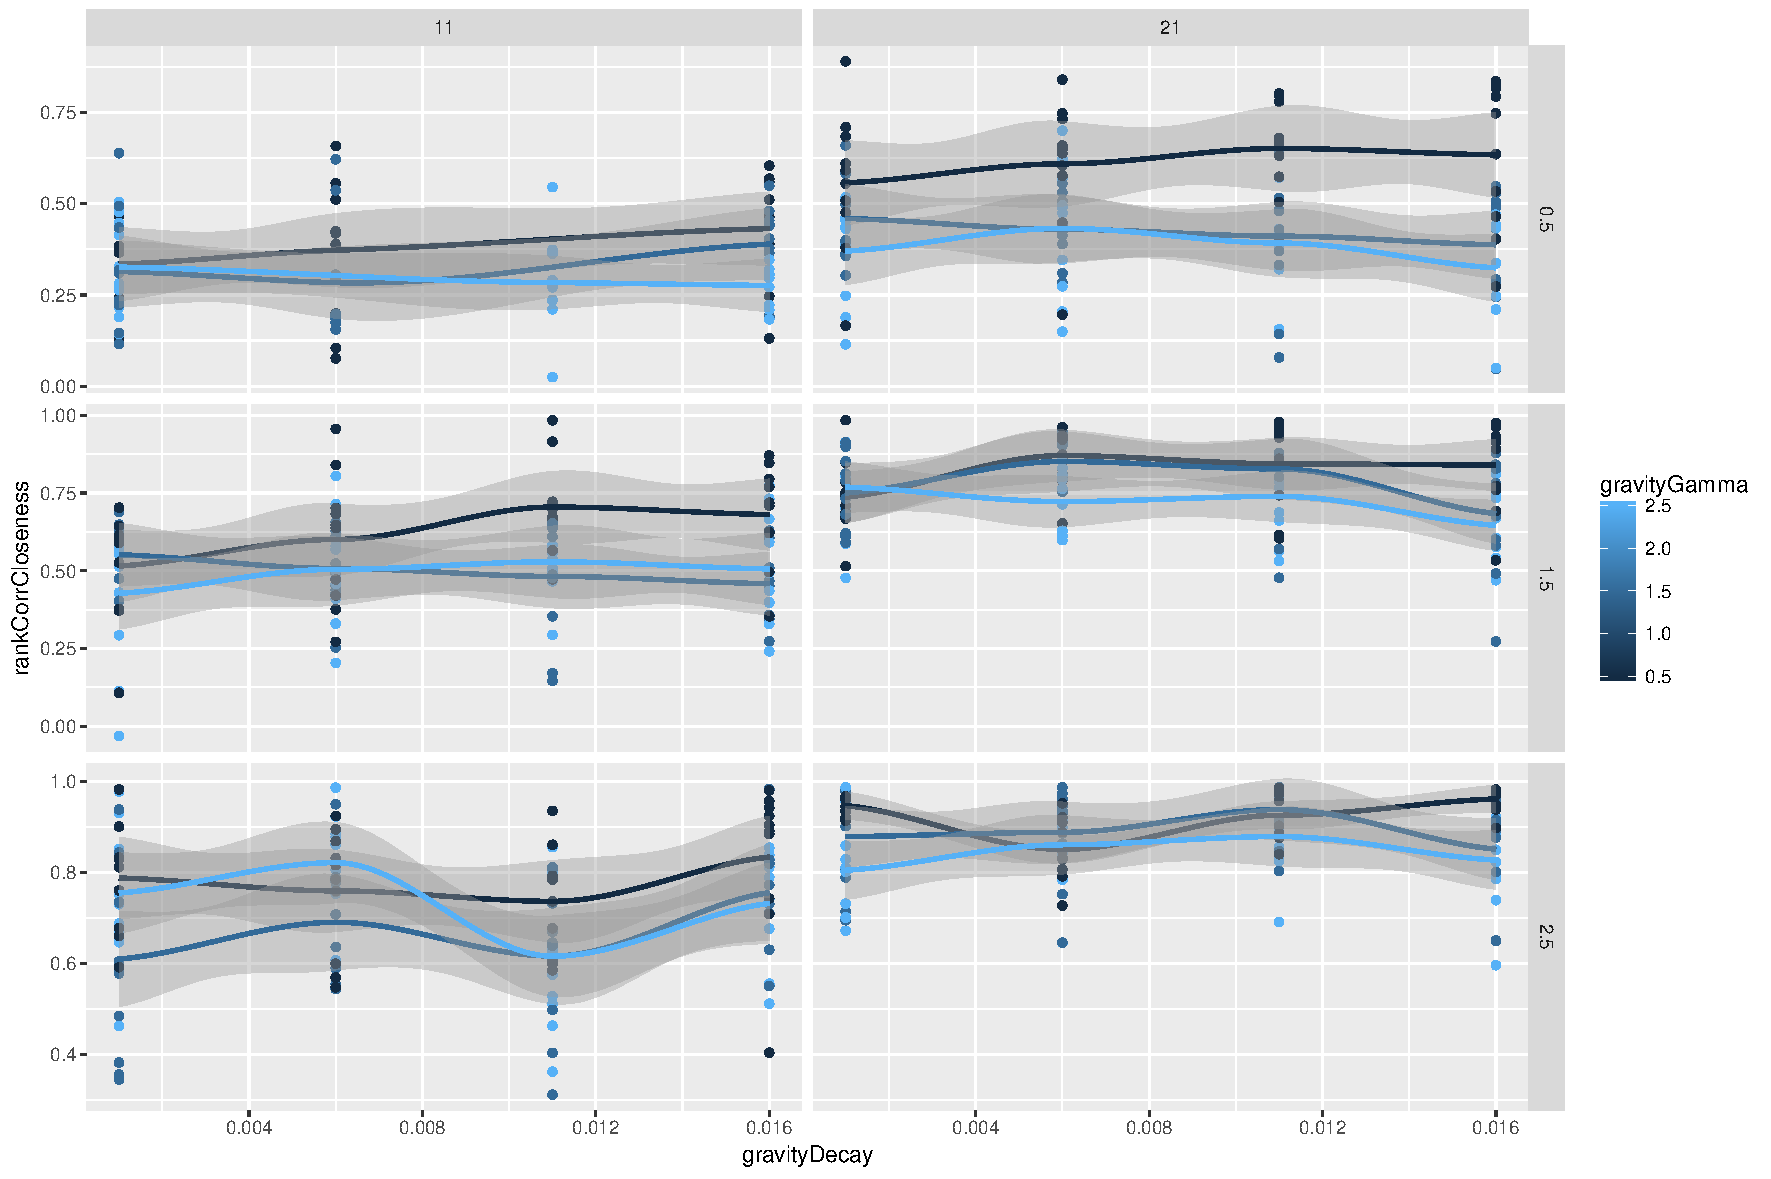
\includegraphics[width=0.48\textwidth]{Figures/MacroCoEvolExplo/rankCorrCloseness_synthRankSize1_5_networkSpeed10}\\
	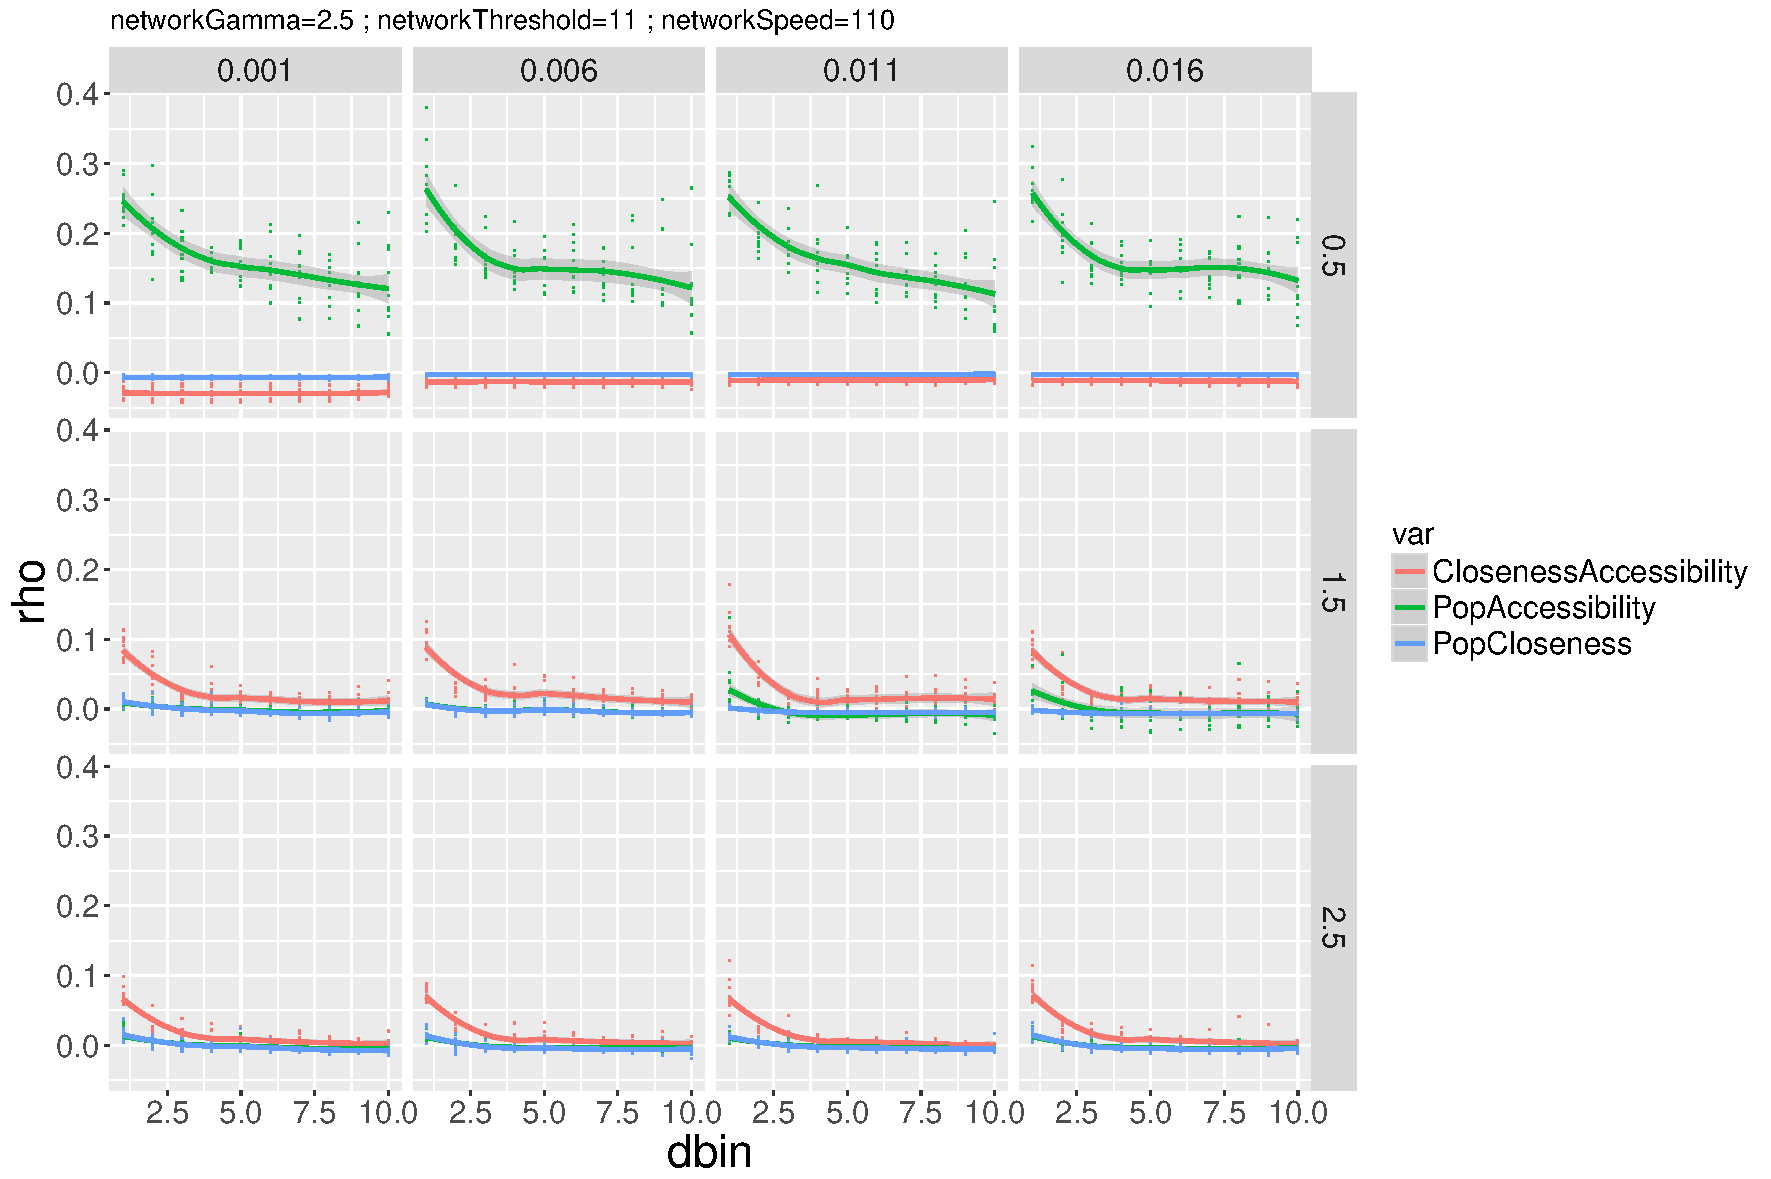
\includegraphics[width=0.48\textwidth]{Figures/MacroCoEvolExplo/distcorrs_networkGamma2_5_networkThreshold11_networkSpeed110}
	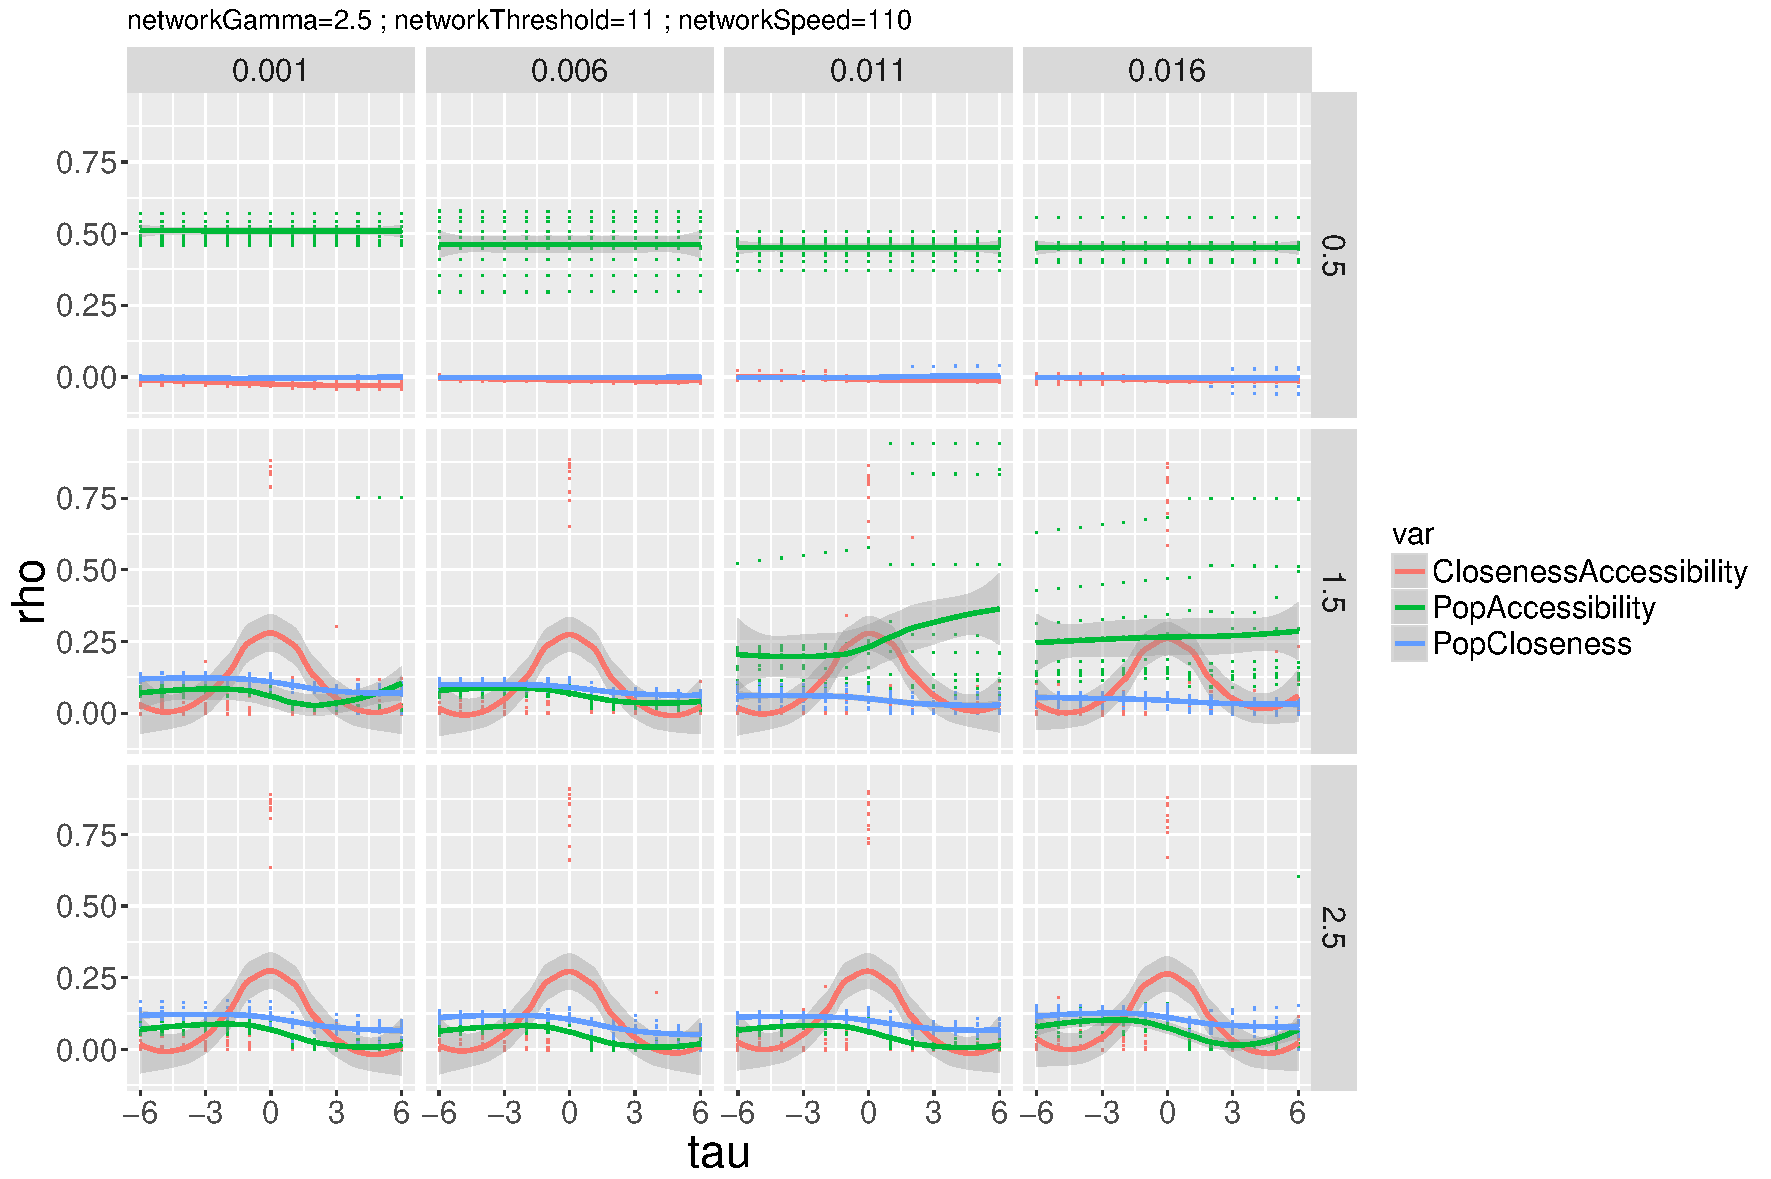
\includegraphics[width=0.48\textwidth]{Figures/MacroCoEvolExplo/laggedcorrs_networkGamma2_5_networkThreshold11_networkSpeed110}
	\caption[][Comportement du modèle]{}{\textbf{Comportement du modèle.} \textit{(Haut Gauche)} Trajectoires temporelles de l'entropie des accessibilités ; \textit{(Haut Droite)} Correlation de rang pour la closeness ; \textit{(bas Gauche)} Correlations en fonction de la distance ; \textit{(Bas Droite)} Correlations retardées.}
\end{figure}
%%%%%%%%%%%%%%%%







%\subsubsection{Discussion}{Discussion}




















